\chapter{工具原型实现}
本章描述了工具原型的一些关键功能的实现技术,主要包括如何利用Clang库来生成抽象语法树,以及根据抽象语法树来生生成输入程序对应的自动机。最好还描述了如何利用自动机进行日志定位。


\section{工具原型运行环境}
本工具原型使用Python语言实现。因此首先需要安装 Python 3.10.8\cite{python310} 版本的开发和运行此环境。
同时需要安装 Clang 12.0.0\cite{Clang12}库,供工具原型用于生成输入程序的抽象语法树。
安装 Clang库后,通过配置 PYTHONPATH 环境变量使其指向 Clang 的 Python 绑定模块 Clang.cindex,使得Python可以找到并使用 Clang 的相关功能。
同时还需要安装名为NetworkX\cite{networkx}的Python库。该库被用于一个用于创建和操作复杂网络的数据结构。

\section{关键功能实现}
本工具原型的关键功能包括如下几个部分:
\begin{enumerate}
    \item 使用Clang的Python库,将C语言程序转换为相应的抽象语法树;
    \item 递归地解析抽象语法树,生成相应的不确定有穷自动机(NFA);
    \item 从不确定有穷自动机出发,从中抽象掉无关信息,仅仅保留日志记录代码的信息,生成确定有穷状态自动机(DFA);
    \item 利用上述的DFA来解析日志序列,获取程序运行信息。
\end{enumerate}
在本小节中将逐个描述这些功能的实现方法。

\subsection{从C语言程序到AST树的转换方法}
对于给定的C语言待分析文件,
工具原型调用cindex模块生成并获取其AST。
其中cindex模块提供了Clang索引库的接口,如章节2.1所言,这个接口用Python封装了
Clang的C语言API,它能使工具原型用与C语言API相似的方式调用Clang来解析源文件。

图\ref{生成C语言程序的AST}的代码用于处理输入文件,生成Clang-AST\\
\begin{figure}[ht]
\centering
\begin{minipage}{12cm}
\begin{lstlisting}
index = cx.Index.create(excludeDecls=True)
tu = index.parse('main.cpp', args=['-std=c'])
pprint(("diags", [get_diag_info(d) for d in tu.diagnostics]))
\end{lstlisting}
\end{minipage}
\caption{生成C语言程序的AST}
\label{生成C语言程序的AST}
\end{figure}

首先工具原型创建了一个类型为Index的对象,该对象提供了cindex模块的主接口,
其主要作用是提供读取和解析翻译单元的接口,并
设置参数 excludeDecls=True,告诉Clang在索引中排除不需要的声明。
这可以减少内存使用并提高性能。

其次,工具原型使用Clang的解析器来解析C语言程序,这将调用Index的parse方法,
从给定的源代码文件加载翻译单元,
并返回一个TranslationUnit对象(tu),其中翻译单元是生成的AST树的根节点。
tu代表了解析源文件的翻译单元,其中 args=['-std=c']参数
指定了使用C语言标准进行解析,
这意味着代码将根据C语言标准的特性和规则进行分析。

最后,工具原型将调用tu中的diagnostics方法,这将返回一个在解析翻译单元时生成的诊断信息列表。
这些诊断信息可以包括错误、警告和信息提示。

\subsection{从根节点解析AST,生成初步的NFA的方法}
当得到了Clang生成的翻译单元,也就是AST树的根节点后,工具原型将从根节点遍历所有的AST节点
,找到每一个代表函数定义的节点。

所以用图\ref{递归遍历AST树,寻找所有的函数定义}所示的递归过程,从AST树的根结点出发,可以递归遍历整个AST树,找到所有函数定义,并对每个函数定义的AST结点生成相应的自动机(Automaton类的对象)。\\

\begin{figure}[ht]
\centering
\begin{minipage}{10cm}
\begin{lstlisting}
traverse(Cursor):
    if 节点类型 是 FUNCTION_DECL:
        if 节点 is 函数定义:
            记录函数出口,入口
            生成该函数节点的自动机(Automaton类)

    # 遍历下一层次的节点
    对当前AST节点的每个下一层次的节点:
        递归调用traverse

\end{lstlisting}
\end{minipage}
\caption{递归遍历AST树,寻找所有的函数定义}
\label{递归遍历AST树,寻找所有的函数定义}
\end{figure}

首先,程序接受一个AST节点的指针(cindex.Cursor)作为参数。在首次调用此递归函数时,该AST节点为上一步生成的翻译单元(TranslationUnit)。

然后,工具原型便判断该节点的类型是否为FUNCTION\_DECL且
节点代表的语句为函数定义,如果是,则提取该函数定义的函数体,
并构造自动机;反之则不做处理。
同时,工具原型还要维护Graph类中的map类数据结构,将得到的函数名和入口出口存入其中。

最后,工具原型将以所有下一层次的AST节点为输入参数,分别调用traverse函数,以达到递归遍历的效果。\\


对于代表语句的ASTNode,工具原型会生成一个对应的代表自动机的Automaton类的对象。

Automaton类的对象中储存了一个指向AST节点所代表的ASTNode的对象,AST节点的类型kind,
语句起始处的stateNode和语句终止处的endNode,以及两个stateNode之间的连接上的标签,标签的内容代表了AST节点代表的语句的类型。
它还包含了传入的跳转目标breakTgt,continueTgt和returnTgt,其中每一个target都是一个stateNode的对象。\\

下面,作者将结合代码,对生成自动机(如图\ref{Auto类的初始化})这一过程进行详细的介绍:

对于一个待生成自动机的AST节点,工具原型会首先初始化一个Automaton类的对象,
代表一个自动机。
Automaton类对象的初始化过程为即将执行的自动机构造过程设置了一些初始值和相关的参数,包括自动机的开始状态和结束状态,以及该AST结点对应的语句中包含的break、continue、return语句的跳转目标信息。\\
\begin{figure}[ht]
\centering
\begin{minipage}{12cm}
\begin{lstlisting}
__init__(cursor: Cursor,breakTgt,continueTgt):
    self.cursor = cursor
    设置break,continue和return的跳转目标
    为stateNode和endNode生成start和end状态
    ...
\end{lstlisting}
\end{minipage}
\caption{Auto类的初始化}
\label{Auto类的初始化}
\end{figure}

大多数情况下,如果AST节点并不需要工具原型提供跳转目标,当工具原型想要为该AST节点创建一个自动机(Automaton类)时,只需要把相应的AST节点自身传入init函数即可。
但是,当AST节点需要工具原型提供跳转目标时,
为了能正确的表示有关跳转的控制流信息,工具原型应该保证生成的自动机能够表示程序运行时可能的执行序列,
所以,工具原型将为需要的AST节点提供return,break和continue语句所需的三个跳转目标,也就是三个stateNode,具体实现如下:
\begin{itemize}
    \item 对于return语句的跳转目标,工具原型需要判断当前AST节点是否为函数体,
若为函数体,则将returnTgt设置为当前AST节点的endNode,
若不是函数体,则继承上一层次的AST节点生成的Automaton类对象中的returnTgt。
    \item 对于break,continue语句,因为代表它们跳转目标的stateNode是在上一层次的AST节点中,
而这些跳转目标,对于break,continue语句在初始化自动机时是未知的,所以工具原型还需要
在生成上一层次的AST节点(如for,while节点)的自动机时,正确传入相应的跳转目标,
然后等到生成下一层次的自动机时,再将其中需要跳转目标的自动机连接到相应的跳转目标(breakTgt或continueTgt)上。具体的说,上一层次的节点在调用buildAutomaton后改变了breakTgt或continueTgt,则会将新的跳转目标传入下一层次的节点;反之,下一层次的节点则直接继承上一层次节点的跳转目标。
\end{itemize}

最后,初始化函数会生成两个初始state,作为自动机的入口状态和出口状态。\\


当AST节点对应的初始化完成后,对于复杂语句,工具原型还需要进一步
根据节点类型,生成该自动机的内部层次结构。具体的说,就是生成下一层次的AST节点的
的自动机,并处理好它们之间的层次关系。
所以,在Automaton类对象初始化之后,还需要调用buildAutomaton方法。\\

图\ref{生成下一层次的AST节点的自动机}是Automaton类的方法 buildAutomaton,它将会根据AST节点类型,生成下一层次的AST节点的自动机,
并最终生成该自动机的内部层次结构。其中breakTgt,continueTgt等信息,均记录在对象self的成员变量中,可供buildAutomaton使用。
\\
\begin{figure}[ht]
\centering
\begin{minipage}{10cm}
\begin{lstlisting}
buildAutomaton(breakTgt,continueTgt): 
    获取下一层次的节点的列表 cursorChilds
    #对各种节点类型的判断及处理
    ...
    elif self.cursor.kind == CursorKind.COMPOUND_STMT:
    ... ...
    elif self.cursor.kind == CursorKind.FOR_STMT:
    ... ...
    elif self.cursor.kind == CursorKind.WHILE_STMT:
    ... ...
    elif self.cursor.kind == CursorKind.IF_STMT:
    ... ...
    elif self.cursor.kind == CursorKind.SWITCH_STMT:
    ...
    
\end{lstlisting}
\end{minipage}
\caption{生成下一层次的AST节点的自动机}
\label{生成下一层次的AST节点的自动机}
\end{figure}

对于整个AST的分析,都建立在递归调用buildAutomaton上的,当某一个Automaton类对象调用该函数时,它便会生成该对象的下一层次所有节点的Automaton类的对象,具体步骤为:
\begin{enumerate}
	\item 判断该AST节点的类型,并获取下一层次的AST节点。
	\item 调用每个下一层次的AST节点的buildAutomaton方法,递归生成下一层次的节点的自动机结构。
	\item 根据节点类型,处理下一层次的AST节点之间的层次关系,并以这种更细致的层次结构重新连接 start\_state-->end\_state

\end{enumerate}

递归调用buildAutomaton,从而生成自动机的过程,是整个工具原型中的重要环节。
下面将对buildAutomaton方法中,关于各种类型的AST节点的处理进行详细解释。

\subsubsection{对break,continue和return语句的处理}
图\ref{跳转语句处理}是对break,continue和return节点的处理的伪代码。因为程序的控制流会在
这些语句发生跳转,所以,工具原型需要将AST节点对应的自动机连接到跳转目标上,
其中每一个跳转目标都是一个stateNode类的对象。

\begin{figure}[ht]
\centering
\begin{minipage}{12cm}
\begin{lstlisting}
buildAutomaton(breakTgt,continueTgt): 
    if self.cursor.kind == CursorKind.BREAK_STMT:            
        从break自动机的endNode连接到已传入的breakTgt
    elif self.cursor.kind == CursorKind.CONTINUE_STMT:
        从continue自动机的endNode连接到已传入的continueTgt
    elif self.cursor.kind == CursorKind.RETURN_STMT:
        从return自动机的endNode连接到已传入的returnTgt
\end{lstlisting}
\end{minipage}
    \caption{跳转语句处理}
    \label{跳转语句处理}
\end{figure}

因为工具原型在生成这些跳转语句的上层次节点的自动机时,已经分配好了跳转目标,所以在这里工具原型只需将跳转语句的自动机连接到
已经传入的跳转目标上即可。

\begin{comment}
\subsubsection{对表达式语句的处理}
图\ref{表达式处理}是对表达式的节点的处理的伪代码。

\begin{figure}[ht]
\centering
\begin{minipage}{10cm}
\begin{lstlisting}
buildAutomaton(breakTgt,continueTgt): 
    elif self.cursor.kind == CursorKind.DECL_STMT:
        ...
    elif self.cursor.kind == CursorKind.BINARY_OPERATOR:
        ...
    elif self.cursor.kind == CursorKind.UNARY_OPERATOR:
        ...
\end{lstlisting}
\end{minipage}
    \caption{表达式处理}
    \label{表达式处理}
\end{figure}
\end{comment}


表达式代表的AST节点均为简单的结构,所以工具原型只是为其添加了标签,方便展示中间结果。

\subsubsection{对函数调用的处理}
图\ref{函数调用处理}是对函数调用的节点的处理的伪代码,工具原型用不同方式处理了日志函数和其他普通的函数。

\begin{figure}[ht]
\centering
\begin{minipage}{9cm}
\begin{lstlisting}
buildAutomaton(breakTgt,continueTgt): 
    elif self.cursor.kind == CursorKind.CALL_EXPR:
        if 函数名为"log":
            对日志函数的处理
        else:
            对普通函数调用的处理
\end{lstlisting}
\end{minipage}
    \caption{函数调用处理}
    \label{函数调用处理}
\end{figure}

当AST节点是一般函数的调用时,工具原型需要先来到到储存函数表的map中,查找对应函数的入口和出口,
并将函数的入口和出口连接到函数调用的位置所在的上文和下文。

当AST节点是log日志函数的调用时,工具原型获取log函数的参数,并将其添加到自动机的输入字
符集中,最后将参数作为标签,添加到边上。

\subsubsection{对顺序结构(复合语句)的处理}
图\ref{顺序结构处理}是对顺序结构的处理的伪代码,这将生成所有下一层次的节点的自动机并按照顺序连接。\\
\begin{figure}[ht]
\centering
\begin{minipage}{14cm}
\begin{lstlisting}
buildAutomaton(breakTgt,continueTgt): 
    elif self.cursor.kind == CursorKind.COMPOUND_STMT:
        对于下一层次的的每一个节点:  
            生成下一层次的节点的Automaton类的对象
            以从后往前的顺序,连接每一个下一层次的节点的Automaton类的对象
\end{lstlisting}
\end{minipage}
    \caption{顺序结构处理}
    \label{顺序结构处理}
\end{figure}

顺序结构会以类型为compound statement(复合语句)的AST节点存在,生成到源程序的AST树上。对于这类AST节点,
它的下一层次的AST节点生成的自动机需要按照顺序依次连接,最后连复合语句回该节点生成的自动机。

\begin{figure}[htbp]
	\centering
	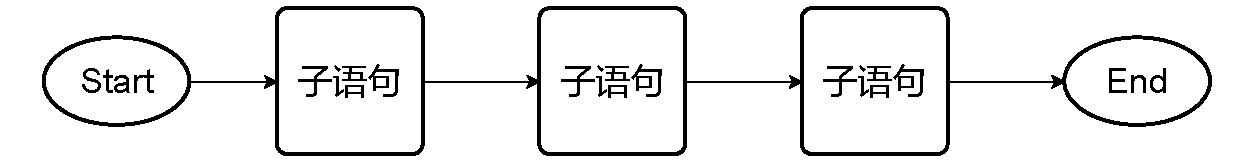
\includegraphics[width=1\textwidth]{pictures/顺序结构.pdf}
	\caption{顺序结构}
	\label{fig:顺序结构}
\end{figure}

图\ref{fig:顺序结构}是顺序结构的程序控制流图。
当复合语句中存在跳转语句时,工具原型需要正确提供跳转目标,但是如果正常地从前往后生成,便可能
出现跳转目标还未生成,工具原型无法提供的情况,所以工具原型在实现上选择了反向连接,如此便保证了所有跳转目标都能在被需要之前生成。


\subsubsection{对for结构的处理}

 \begin{figure}[htbp]
	\centering
	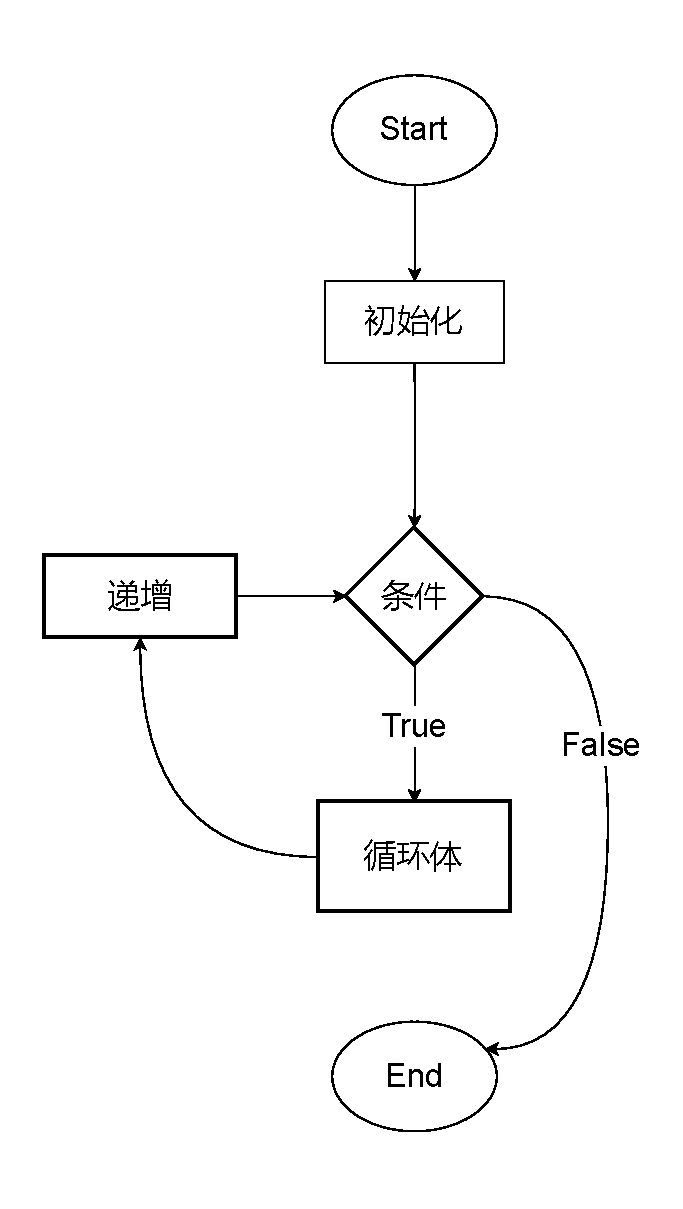
\includegraphics[width=0.4\textwidth]{pictures/for结构.pdf}
	\caption{for的控制流图}
	\label{fig:for的控制流图}
\end{figure}

图\ref{fig:for的控制流图}是for语句的程序控制流图,其中for语句的初始化语句,条件语句,递增语句均有可能为空。
根据C语言的语义,for语句首先执行初始化语句,接着计算条件语句。如果条件表达式为假,则for语句执行结束;如果条件表达式的值为真,那么继续执行循环体中的语句。循环体执行完毕后,程序将执行递增语句,最后返回到条件表达式的开始处继续执行。

for语句中的break和continue语句需要特殊处理:循环体中的break语句执行之后将结束for语句的执行;而continue语句执行之后,程序将转到条件语句处继续执行。即
工具原型在循环体内部处理 break 语句时,需要将该 break 语句对应的
自动机的出口连接到for语句自动机的出口; 在处理 continue 语句时,需要将 continue 语句的自动机的出口连接
到连接到条件语句自动机的入口。\\

\begin{figure}[ht]
\centering
\begin{minipage}{16cm}
\begin{lstlisting}[language=Python]
buildAutomaton(breakTgt,continueTgt): 
    解析for节点,获取该节点的下一层次的节点存在与否的情况。
    根据解析结果,分别生成下一层次的节点的自动机或者代表空节点的自动机:
        获取init的AST节点cond,并构造生成init的自动机initAutomaton
        获取condition的AST节点cond,并构造生成condition的自动机condAutomaton
        获取increasement的AST节点incAutomaton,并构造生成increasement的自动机incAutomaton
    获取statements的AST节点stmts
    stmtsAutomaton = Automaton()        #为循环体初始化一个Automaton类的对象
    stmtsAutomaton.buildAutomaton(stmts,breakTgt=self.end_state,continueTgt=condAutomaton.start_state)     
    #构造statements的自动机stmtsAutomaton
    按照程序控制流图,将for语句中不同部分的自动机连接起来
\end{lstlisting}
    \caption{for结构处理}
    \label{for结构处理}
\end{minipage}
\end{figure}


图\ref{for结构处理}是对for类型节点的处理的伪代码。
工具原型首先判断下一层次中init,condition,increasement三个位置的AST节点的存在与否,生成初始化init的自动机initAutomaton,条件表达式cond的自动机condAutomaton和递增语句的自动机incAutomaton:
\begin{itemize}
    \item 对于存在的AST节点,工具原型将先获取所在位置的AST节点接着,工具原型将为该AST节点初始化一个Automaton类的对象,生成它的自动机。
    \item 对于不存在的AST节点,工具原型将专门初始化一个类型为“empty”的空节点的自动机,用于填充空缺的节点,保持for语句的自动机原有的层次结构。
\end{itemize}

下一步,工具原型将先获取for语句中的statements的AST节点stmts。然后为stmts初始化一个Automaton类的对象stmtsAutomaton.
因为 for 语句的循环体中的 break 将中止 for 语句的执行,工具原型应该将for语句的endNode作为循环体中的break语句的跳转目标(breakTgt)。
同样的,因为 for 语句的循环体中的continue将开始下一轮的循环,工具原型应该将条件表达式对应的NFA的startNode作为循环体中的continue语句的跳转目标(continueTgt)。



最后调用buildAutomaton方法递归生成stmtsAutomaton的不确定自动机。并按照程序控制流图,将for语句中不同部分的自动机连接起来:
\begin{itemize}
    \item for语句的自动机的入口连接到initAutomaton的入口;
    \item initAutomaton的出口连接到condAutomaton的入口;
    \item condAutomaton的出口将以“True”的标签连接到stmtsAutomaton的入口,同时以“False”的标签连接到for语句的自动机的入口;
    \item stmtsAutomaton的出口将连接上incAutomaton的入口;
    \item incAutomaton的出口将连接上condAutomaton的入口。
\end{itemize}



\subsubsection{对while结构的处理}
 \begin{figure}[htbp]
	\centering
	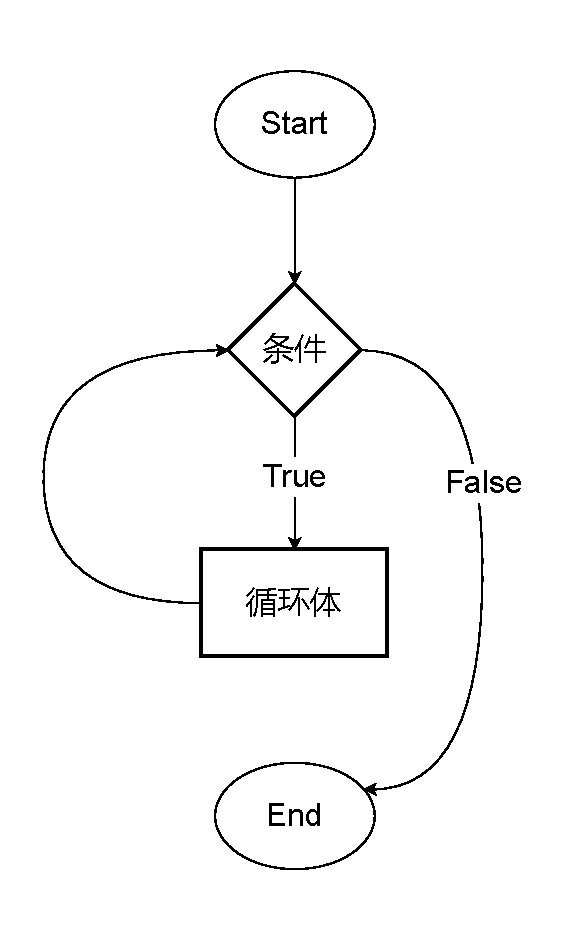
\includegraphics[width=0.4\textwidth]{pictures/while结构.pdf}
	\caption{while的控制流图}
	\label{fig:while结构}
\end{figure}

图\ref{fig:while结构}是while语句的程序控制流图。
根据C语言的语义,while语句首先计算条件语句。如果条件表达式为假,则while语句执行结束;如果条件表达式的值为真,那么继续执行循环体中的语句。循环体执行完毕后,程序将返回到条件表达式的开始处继续执行。

while语句中的break和continue语句需要特殊处理:循环体中的break语句执行之后将结束while语句的执行;而continue语句执行之后,程序将转到条件语句处继续执行。即
工具原型在循环体内部处理 break 语句时,需要将该 break 语句对应的
自动机的出口连接到while语句自动机的出口; 在处理 continue 语句时,需要将 continue 语句的自动机的出口连接
到连接到条件表达式自动机的入口。\\

\begin{figure}[ht]
	\centering
\begin{minipage}{16cm}
\begin{lstlisting}
buildAutomaton(breakTgt,continueTgt): 
    获取condition的AST节点cond,并构造生成condition的自动机condAutomaton
    获取statements的AST节点stmts
    stmtsAutomaton = Automaton()        #为循环体初始化一个Automaton类的对象
    stmtsAutomaton.buildAutomaton(stmts,breakTgt=self.end_state,continueTgt=condAutomaton.start_state)     
    #构造statements的自动机stmtsAutomaton
    按照程序控制流图,将while语句中不同部分的自动机连接起来
\end{lstlisting}
\end{minipage}
    \caption{while语句的处理}
    \label{while结构处理}
\end{figure}

图\ref{while结构处理}是对while语句处理的伪代码,其中while语句的条件节点必定不为空。
工具原型将先获取while语句中的condition的AST节点cond和statements的AST节点stmts。然后为条件表达式cond生成自动机condAutomaton(它是Automaton类的一个对象).

下一步,工具原型将先获取while语句中的statements的AST节点stmts。然后为stmts初始化一个Automaton类的对象stmtsAutomaton.
因为 while 语句的循环体中的 break 将中止 while 语句的执行,工具原型应该将while语句的endNode作为循环体中的break语句的跳转目标(breakTgt)
同样的,因为 while 语句的循环体中的continue将开始下一轮的循环,工具原型应该将条件表达式对应的NFA的startNode作为循环体中的continue语句的跳转目标(continueTgt)。

最后按照程序控制流图,将while语句中不同部分的自动机连接起来:
\begin{itemize}
    \item while语句的自动机的入口连接到condAutomaton的入口;
    \item condAutomaton的出口将以“True”的标签连接到stmtsAutomaton的入口,同时以“False”的标签连接到while语句的自动机的入口;
    \item stmtsAutomaton的出口将连接上condAutomaton的入口。
\end{itemize}

\subsubsection{对if结构的处理}

 \begin{figure}[htbp]
	\centering
	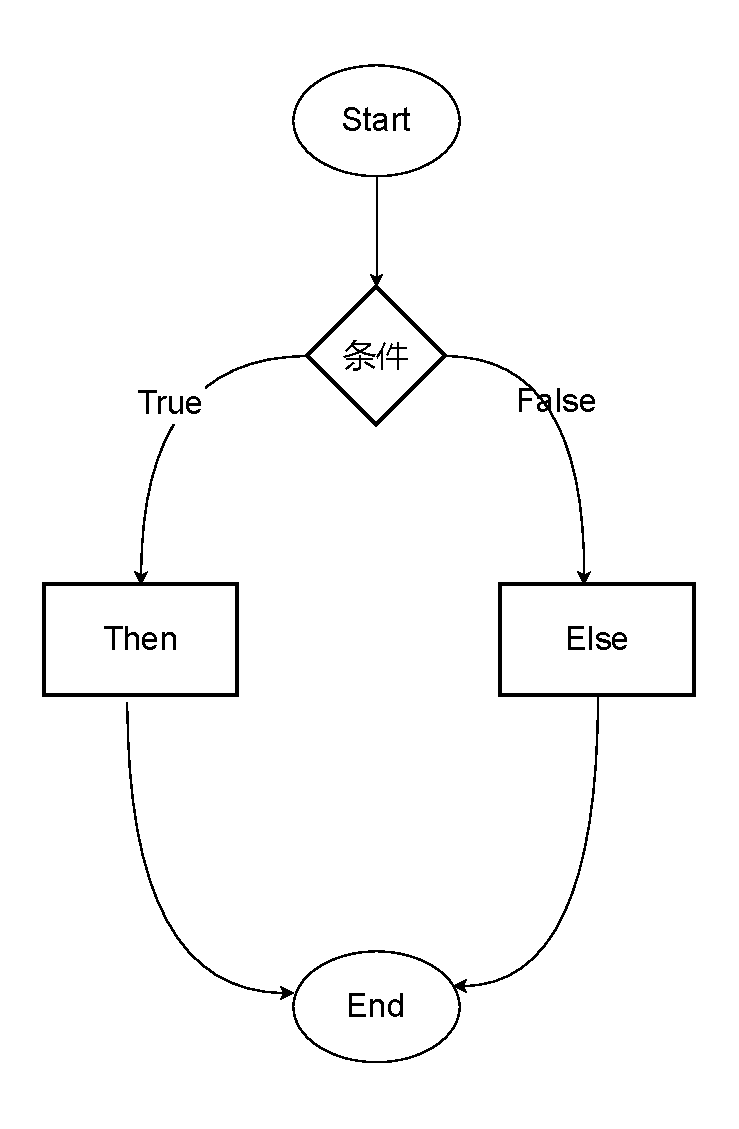
\includegraphics[width=0.4\textwidth]{pictures/if结构.pdf}
	\caption{if的控制流图}
	\label{fig:if的控制流图}
\end{figure}

图\ref{fig:if的控制流图}是if语句的程序控制流图。
根据 C语言 的语义,if语句首先计算条件语句。如果条件表达式为假,
则 执行if语句中的then分支;如果条件表达式的
值为真,那么继续执行执行if语句中的else分支。

if 语句中的 break 和 continue 语句不需要特殊处理。
在为 if 语句中的then分支和else分支生成 NFA 时,工具原型应该将 if 语句上一层次的语句自动机中记录的跳转目标(breakTgt,continueTgt)直接继承给if 语句中的then分支和else分支,作为 if 语句中的then分支和else分支 break语句和continue语句的跳转目标。即工具原型在then分支和else分支内部处理 break和continue 语句时,需要将该 break 语句对应的自动机的出口连接到上一层次的语句自动机的breakTgt和continueTgt.

\begin{figure}[ht]
	\centering
\begin{minipage}{16cm}
\begin{lstlisting}
buildAutomaton(breakTgt,continueTgt): 
    获取condition的AST节点cond,并构造生成condition的自动机condAutomaton
    获取then分支的AST节点then-branch
    thenAutomaton = Automaton(); #为then-branch初始化一个Automaton类的对象
    thenAutomaton.buildAutomaton(then,breakTgt=self.breakTgt,continueTgt=self.continueTgt)    
    #构造statements的自动机stmtsAutomaton
    if 该ASTNode代表一个带有else分支的if语句:
        获取else分支的AST节点else-branch
        elseAutomaton = Automaton(); #为else-branch初始化一个Automaton类的对象
        elseAutomaton.buildAutomaton(else,breakTgt=self.breakTgt,continueTgt=self.continueTgt)    
        #构造else的自动机elseAutomaton
        按照程序控制流图,将if语句中不同部分的自动机连接起来
    else:
        按照程序控制流图,将没有else分支的if语句中不同部分的自动机连接起来
\end{lstlisting}
\end{minipage}
    \caption{if结构处理}
    \label{if结构处理}
\end{figure}

图\ref{if结构处理}是对if结构的处理的伪代码。
工具原型将先获取if语句中的condition的AST节点cond和then分支的AST节点then。
然后为条件表达式 cond 生成自动机 condAutomaton(它是 Automaton 类的一个
对象);同时为 then 初始化一个 Automaton 类的对象 thenAutomaton,继承if自动机本身的breakTgt和continueTgt,
最后调用 buildAutomaton 方法递归生成 thenAutomaton 的不确定自动机。

下一步,工具原型对if的AST节点的下一层次节点中有else分支和没有else分支的两种情况做出不同的处理,最后按照程序控制流图,将if语句中不同部分的自动机连接起来:
\begin{itemize}
    \item 当while节点下一层次的节点数量大于2时,说明while节点存在else分支。
    工具原型将获取else分支的AST节点else,
    并为else分支初始化一个Automaton类的对象elseAutomaton,继承if节点本身的breakTgt和continueTgt,最后调用 buildAutomaton 方法递归生成 elseAutomaton 的不确定自动机。
    \begin{itemize}
        \item if 语句的自动机的入口连接到 condAutomaton 的入口;
        \item condAutomaton 的出口将以“True”的标签连接到 thenAutomaton 的入口;
        \item thenAutomaton 的出口连接到 if 语句的自动机的出口。
        \item condAutomaton 的出口将以“False”的标签连接到 elseAutomaton 的入口;
        \item elseAutomaton 的的出口连接到 if 语句的自动机的出口。
    \end{itemize}
    \item 当while节点下一层次的节点数量不大于2时,说明while节点不存在else分支。
        \begin{itemize}
        \item if 语句的自动机的入口连接到 condAutomaton 的入口;
        \item condAutomaton 的出口将以“True”的标签连接到 thenAutomaton 的入口;
        \item thenAutomaton 的出口连接到 if 语句的自动机的出口。
        \item condAutomaton的出口将以“False”的标签连接到if语句的自动机的出口。
    \end{itemize}
\end{itemize}

\subsubsection{对switch结构的处理}


\begin{figure}[htbp]
	\centering
	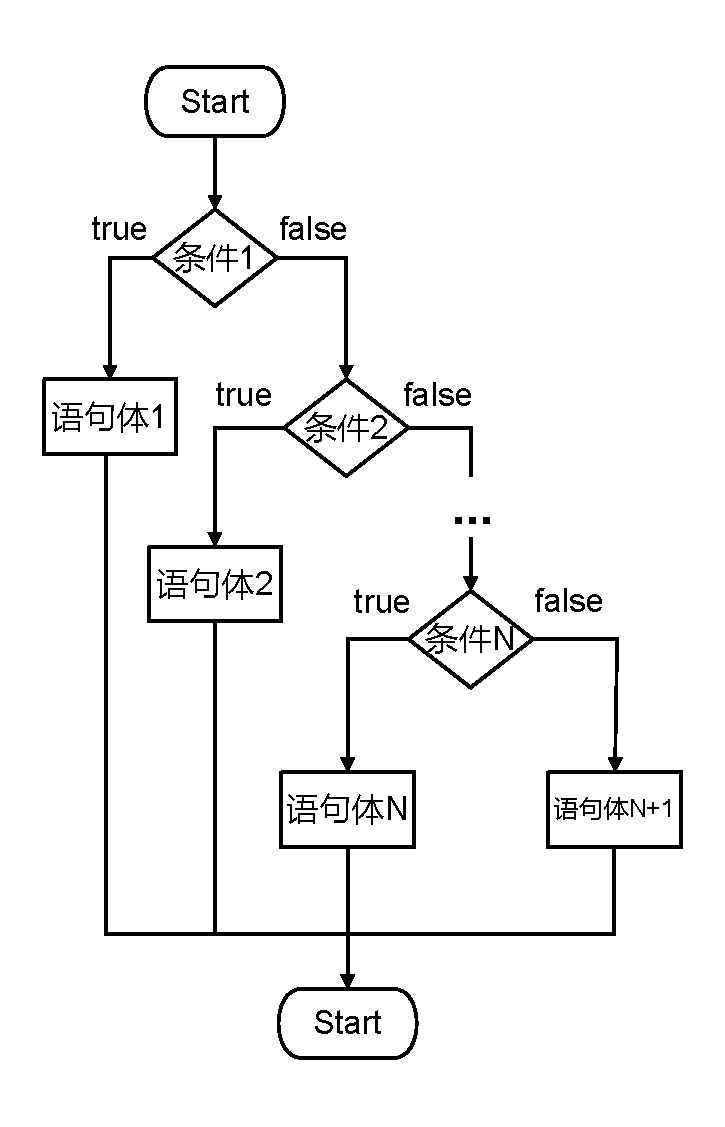
\includegraphics[width=0.5\textwidth]{pictures/switch结构.pdf}
	\caption{switch结构}
	\label{fig:switch结构}
\end{figure}

图\ref{fig:switch结构}是switch语句的程序控制流图。
图4-11是 switch 语句的程序控制流图。根据 C语言 的语义,switch 语句首先计算控制表达式的值。然后,该值与 case 标签所指定的值进行比较。如果找到与控制表达式的值匹配的 case 标签,程序将从该 case 标签开始执行对应的语句,执行完毕后,程序将继续匹配下一个case标签。如果没有匹配的 case 标签,且存在 default 标签,那么程序将执行 default 标签处的语句;如果没有 default 标签,则 switch 语句执行结束而不执行任何语句。

在 switch 语句中,break 语句需要特殊处理,continue语句则不需要:当 case 或 default 语句块中遇到 break 语句时,程序将跳出 switch 语句的执行。因此,在为 switch 语句的case生成 NFA 时,工具原型应该将 switch 语句的出口作为case中的 break 语句的跳转目标(breakTgt),将 switch 语句
上一层次的语句自动机中记录的 continue语句的跳转目标(continueTgt)直接继承给 case 语句,作为 case 语句中的 continue 语句的跳转目标。即工具原型在case内部处理 break 语句时,需要将该 break 语句对应的自动机的出口连接到 switch 语句自动机的出口;
在case中的 continue 语句时,需要将 continue 语句的自动机的出口连
接到上一层次的语句自动机的 continueTgt。

 \begin{figure}[htbp]
	\centering
\begin{minipage}{16cm}
\begin{lstlisting}
buildAutomaton(breakTgt,continueTgt): 
    #对switch结构的处理
    获取包含多个case的复合语句的AST节点cases
    casesAutomaton = Automaton()        #为cases初始化一个Automaton类的对象
    casesAutomaton.buildAutomaton(cases,breakTgt=self.end_state,continueTgt,self.continueTgt)    
    #构造cases的自动机casesAutomaton
    按照程序控制流图,将swich语句中不同部分的自动机连接起来
    ... ...
    #对单个case结构的处理
    获取condition的AST节点cond,并构造生成condition的自动机condAutomaton
    获 取statements的AST节点stmts
    stmtsAutomaton = Automaton(); #为statements初始化一个Automaton类的对象
    stmtsAutomaton.buildAutomaton(stmts,breakTgt=cases.breakTgt,continueTgt=cases.continueTgt)     
    #构造statements的自动机stmtsAutomaton
    按照程序控制流图,将单个case语句中不同部分的自动机连接起来
\end{lstlisting}   
\end{minipage}
    \caption{对switch结构和单个case结构的处理}
    \label{对switch结构和单个case结构的处理}
\end{figure}

图\ref{对switch结构和单个case结构的处理}是对switch结构和单个case结构的处理的伪代码。
工具原型将先获取switch语句中的包含多个case的复合语句的AST节点cases, 为cases初始化一个 Automaton 类的对象 casesAutomaton,
并设置 breakTgt和 continueTgt,最后调用buildAutomaton方法递归生成casesAutomaton的不确定自动机。
因为cases的AST节点的类型为“COMPOUND\_STMT”,buildAutomaton方法将会把case节点视为复合语句节点,以处理顺序结构的方式处理cases节点,按照程序控制流图,将cases内的每个case按照顺序连接:
\begin{itemize}
    \item switch语句的自动机的入口连接到casesAutomaton的入口;
    \item casesAutomaton内的每一个case自动机(caseAutomaton)将依次首尾相连;
    \item casesAutomaton的出口将连接上switch语句的自动机的出口。
\end{itemize}

此外,工具原型还实现了对于单个case语句的处理。工具原型将先获取case语句中的condition的AST节点cond和statements的AST节点stmts。然后为条件表达式cond生成自动机condAutomaton(它是Automaton类的一个对象);同时为stmts初始化一个Automaton类的对象stmtsAutomaton,并继承switch自动机本身的breakTgt和continueTgt,最后调用buildAutomaton方法递归生成stmtsAutomaton的不确定自动机。最后按照程序控制流图,将case语句中不同部分的自动机连接起来,生成caseAutomaton:
\begin{itemize}
    \item case语句的自动机的入口连接到condAutomaton的入口;
    \item condAutomaton的出口将以“True”的标签连接到stmtsAutomaton的入口,同时以“False”的标签连接到case语句的自动机的出口;
    \item stmtsAutomaton的出口将连接上case语句的自动机的出口。
\end{itemize}



\subsection{从初始NFA获取日志函数的输入,最终生成DFA的方法}
当工具原型得到由自动机组成的初始NFA后,还需要对其进一步处理。
因为待分析的日志记录中只有日志函数的输出,所以,需要保证自动机的边上的输入只能来自log日志函数的参数。
因此,工具原型先将无用的标签去掉,使得初始的NFA转为只有合法输入的NFA。
在这种情况下,所有没有标签的边在新的NFA中都被当做空边处理。

接下来,为了实现子集构造法,工具原型实现了一个返回状态的空边闭包的函数

图\ref{返回状态的空边闭包}的函数将返回给定集合的epsilon闭包。\\
 \begin{figure}[htbp]
	\centering
\begin{minipage}{14cm}
\begin{lstlisting}
epsilon_closure(states):
    初始化closure,queue
    当queue不为空时:
        current_state = queue.pop()
        将epsilon_transitions设为从current_state出发的所有空边的目的地
        对于epsilon_transitions中每一个state:
            if state 不在 closure内:
                将state加入queue和closure
    return frozenset(closure)
\end{lstlisting}
    \caption{返回状态的空边闭包}
    \label{返回状态的空边闭包}
\end{minipage}
\end{figure}
这段代码是一个函数epsilon\_closure,它接收一个状态集合作为输入参数。
它的功能是计算从给定的状态集合出发,通过空边可以到达的所有状态,然后返回这些状态的闭包。
代码的执行过程如下:
首先,将输入的状态集合初始化为闭包集合closure,同时将该集合添加到一个队列queue中。
进入循环,只要队列不为空,就执行以下操作:
\begin{itemize}
	\item 弹出队列中的一个状态current\_state作为当前状态。
	\item 找到从当前状态出发的所有空边的目的地,这些目的地的标签为空。将这些目的地添加到列表epsilon\_transitions中,其中列表元素是状态。
	\item 对于每个目的地状态state,如果它不在闭包集合closure中,就将它添加到闭包集合中,并将其加入队列queue中,以便后续继续扩展闭包。
\end{itemize}

循环结束后,闭包集合closure中包含了从输入状态集合出发,通过空边可以到达的所有状态。最后
使用frozenset将其转换成不可变的冻结集合,并作为结果返回。

接下来,工具原型实现了一个NFA到DFA的转换函数(图\ref{子集构造法}),并在其中调用了图\ref{返回状态的空边闭包}的epsilon\_closure函数。

 \begin{figure}[htbp]
	\centering
\begin{minipage}{16cm}
\begin{lstlisting}
NFA2DFA(self):
    将初始的unmarked_states设为main函数的startNode的epsilon闭包
    获取自动机的字符表alphabet
    当 unmarked_states 不为空时:
        current_states = unmarked_states.pop(0)
        对于alphabet中的每一个symbol:
            next_states = set()
            对于current_states中的每一个state:
                寻找通过symbol可以到达的state,并将其epsilon闭包加入next_states
            if next_states不为空:
                if next_state不在DFA中
                    将next_states加入DFA
                    将next_states加入unmarked_states
                连接current_states到next_state,标签为symbol
\end{lstlisting}
\end{minipage}
    \caption{子集构造法}
    \label{子集构造法}
\end{figure}
首先,从NFA的起始状态集合(设定为main函数的入口)开始,使用epsilon\_closure函数计算该状态集合的epsilon闭包,
并将其作为初始状态加入DFA中。
创建一个列表unmarked\_states,用于存储未标记的DFA状态集合(即待处理的状态集合)。
只要unmarked\_states不为空,就循环执行以下操作:
\begin{enumerate}
	\item 弹出unmarked\_states列表的第一个元素(DFA的state),加入当前状态集合current\_states。
	\item  对于输入字符集合中的每个输入符号symbol(也就是日志记录文件中的一条记录),创建一个空集合next\_states,
 用于存储当前状态集合通过
 symbol转换能够到达的状态集合,对于current\_states中的每个状态state,
 找到从state经过symbol转换可以到达的状态集合transitions。
 对于transition\_state中的每个状态,
 计算其epsilon闭包,并将这些状态添加到next\_states集合中。
	\item 如果next\_states非空,则将
 next\_states作为新的DFA状态集合next\_state。
 如果next\_state尚未添加到DFA中,则将其添加为一个新的状态,
 并将其添加到unmarked\_states列表中,以进行后续处理。
 在DFA中添加一条边,从current\_states到next\_state,标记为symbol。
\end{enumerate}
循环结束后,DFA的构建完成,其中每个节点表示一个DFA状态集合,边表示状态之间的转换,标记为输入符号。
\subsection{结合DFA,解析日志序列}
最后一步,工具原型实现了函数runDFA,它可用生成的DFA,解析日志记录。

图\ref{以日志为输入,运行DFA}函数将用DFA解析给定的日志记录,若结果错误(输入不合法或者日志错误),将返回一个空的列表;
否则,返回源程序在运行时,经过的DFA的stateNode的一个列表,这在一定程度上表示了程序的运行路径。\\
 \begin{figure}[htbp]
	\centering
\begin{minipage}{8cm}
\begin{lstlisting}
runDFA(self):
    读取输入文件
    输入字符的合法性检查
    初始化 DFA 的状态 current_state
    维护一个 visited_states 列表
    运行状态转移
    返回走过的state列表,用于后续染色展示
\end{lstlisting}
\end{minipage}
    \caption{以日志为输入,运行DFA}
    \label{以日志为输入,运行DFA}
\end{figure}

首先,这个函数将打开一个名为 loginfo.txt 的文件,
作者假设需要分析的日志就在其中。函数将去除每行的换行符和空白字符,
并读取其中的所有行。接着工具原型将检查每个处理后的字符是否在 DFA 的输入字符集合中,
如果不在,打印错误信息并返回空列表。

其次,将current\_state首先设置为 DFA 的开始状态
(其中必定包含NFA中的main函数的startNode节点)。
将current\_state加入visited\_states的list,
用于记录DFA运行时访问过的所有节点。

对于日志记录中每一行的日志log,工具原型将其看作自动机的一个输入字符,并在当前状态的所有转移边中寻找匹配的边。
检查当前状态的每一条转移边的标签是否与当前输入字符匹配。
如果找到匹配的边,更新 current\_state 为下一个状态,
并将其添加到 visited\_states 中。
如果没有找到匹配的转移边,说明日志记录错误(不可能存在这样的日志序列),打印错误信息并返回空列表。

最后,如果所有输入字符都合法且找到对应的状态转移,
返回运行时访问过的所有节点的列表 visited\_states,工具原型将会把存在于visited\_states中的状态节点染上不同颜色,用于区分展示。\\

在得到了所有日志相关的信息后,工具原型便可对工具原型的运行情况进行进一步的分析。

如果自动机成功运行到了接受状态,工具原型可以根据生成的DFA(如图\ref{fig:日志分析的可视化}),了解它的实际运行过程,比如经过了哪些语句,在选择语句时选择了哪一个分支等等。

如果自动机没有运行到接受状态,而是停在了中间的某个位置,开发人员便可针对
这类情况设计特殊的日志,进行错误分析,以及出错时调用栈的内容。
\begin{enumerate}
    \item 识别错误日志记录:假设每条记录的格式已知,
    并且包含明确的错误标识符(例如,"ERROR"、"EXCEPTION" 等),
    开发人员可以扫描日志内容,找出所有包含这些关键字的日志,进而分析程序的错误是如何生成的。
    \item 解析程序点的位置:假设日志记录中包含有关程序点的信息,如函数名、文件名和行号。
    这些信息通常在错误日志中出现,开发人员可以通过解析错误发生时周围的日志来找到。
    \item 提取错误发生时的调用栈内容:假设开发人员在每个函数的入口处和出口都放置一条
    日志函数代表该函数的调用和退出,这样在程序发生错误后,这些信息会详细列出错误发生时的函数调用顺序,
    开发人员便可以用这类日志函数来判断函数发生错误时的调用栈。
\end{enumerate}

\section{本章小结}
本章深入到工具原型实现的细节,涵盖了工具原型的运行环境配置、关键功能的实现步骤和具体技术细节。

在工具原型运行环境部分,工具原型使用Python 3.10.8作为开发和运行的编程语言,
并安装Clang 12.0.0及其Python绑定模块Clang.cindex。
此外,还需要安装Python库NetworkX用于处理自动机组成的有向图网络。

关键功能实现部分描述了工具原型的核心功能,分为四个主要步骤:
\begin{enumerate}
    \item 从C语言程序生成抽象语法树(AST)。
    \item 递归解析AST,生成初步的非确定有限自动机(NFA)。
    \item 根据NFA获取日志信息,进一步生成确定有限自动机(DFA)。
    \item 结合DFA,解析日志序列。
\end{enumerate}

每个步骤都有详细的伪代码片段和解释,
例如从C语言程序生成AST的过程使用了Clang的接口和Python代码示例,
展示了如何处理不同类型的AST节点来构建NFA。
递归解析AST的过程中,通过Automaton类表示自动机,
并展示了如何处理不同的语句结构(如顺序结构、循环结构、条件结构等)
以及函数调用和控制流语句。

最后,文章描述了从初始NFA获取日志信息并生成DFA的过程,
涉及到epsilon闭包的计算和子集构造法的应用,
以确保工具原型能够准确解析和识别特定的日志信息。


